\documentclass[compress,11pt]{beamer}
%\includeonly{pendel}
\usetheme{Ilmenau}
%\usetheme{fau-4-3}
%\usecolortheme{beaver}
%\beamertemplatenavigationsymbolsempty
\usepackage[ngerman]{babel}
\usepackage{marvosym}
\usepackage{multimedia}
\usepackage[utf8]{inputenc}
\usepackage{amsmath}
\usepackage{amsfonts}
\usepackage{amssymb}
\usepackage{graphicx}
\usepackage{esvect}
%\author{}
\title{EP Gruppe 8}
%\setbeamercovered{transparent}
%\setbeamertemplate{navigation symbols}{}
%\logo{}
%\institute{}
%\date{}
%\subject{}
\usepackage{verbatim}
\begin{document}
\section{Einführung in PID-Regelung}
\subsection{Übersicht über Regelungstypen}
\subsubsection{I-Regler}
\begin{frame}
Übertragungsgleichung:
\begin{equation}
u(t) = K_p \cdot e(t)
\end{equation}
Hierbei sind:
\begin{itemize}
\item $e(t)$: Regelabweichung des Systems (Differenz von Sollwert und Istwert der zu regelnden Größe, bei und die Temperatur)
\item $u(t)$: Stellgröße, die an die Regelstrecke weitergegeben wird, um der Regelabweichung entgegenzuwirken
\item $K_p$: Regler-Parameter, mit dem der Abweichung entgegengewirkt wird
\end{itemize}
\end{frame}
\begin{frame}
\begin{block}{Eigenschaften des P-Reglers}
\begin{itemize}
\item Regelung ist relativ schnell
\item Stellgröße kann schnell hohe Werte annehmen und damit an Begrenzungen des Systems stoßen
\item Sollwert nur durch P-Regelung nicht erreichbar, entweder Näherung von unten oder ungedämpfte Schwingung um die Stellgröße
\end{itemize}
\end{block}

$\Rightarrow$ P-Regler alleine werden nur selten in der Praxis verwendet

\end{frame}
\subsubsection{I-Regler}
\begin{frame}

Übertragungsgleichung:
\begin{equation}
u(t) = K_t \cdot \int_0^t e(\tau) \mathrm{d}x
\end{equation}
Hierbei sind:
\begin{itemize}
\item $e(t)$, $u(t)$ wie oben
\item $K_t$: Regler-Parameter, mit dem der Abweichung entgegengewirkt wird
\end{itemize}
\end{frame}
\begin{frame}
\begin{block}{Eigenschaften des I-Reglers}
\begin{itemize}
\item Regelung ist relativ schnell
\item Stellgröße kann schnell hohe Werte annehmen und damit an Begrenzungen des Systems stoßen
\item Sollwert nur durch P-Regelung nicht erreichbar, entweder Näherung von unten oder ungedämpfte Schwingung um die Stellgröße
\end{itemize}
\end{block}

\end{frame}

\begin{frame}


\subsection{Aufgabe a)}
%Schaltung
\begin{itemize}
\item Metallblock wurde mittels Peltierelement erwärmt
\item Widerstand des Blocks wurde gemessen und in Temeratur umgerechnet
\end{itemize}
Aufgabe war es, mittels Power-Supply den Strom am Peltierelement so zu regeln, dass die Temperatur des Blocks konstant bleibt
\end{frame}
\begin{frame}
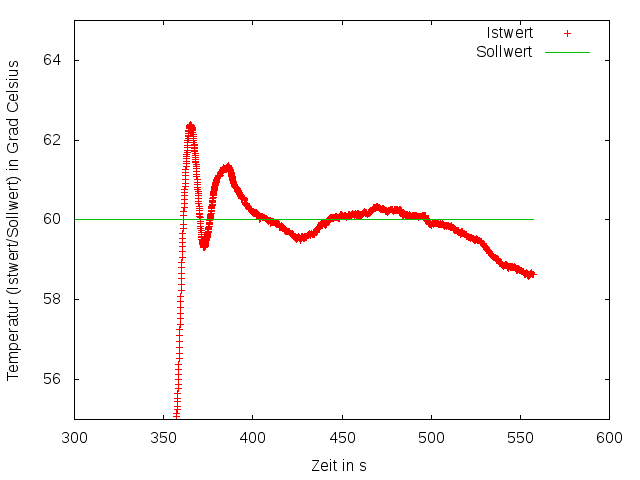
\includegraphics[width=.7\textwidth]{../2aufgabe/2a_T_genauer}\\
Ergebnis der Regelung
\end{frame}
\begin{frame}
\begin{block}{"Vorgehensweise" beim Regeln}
\begin{itemize}
\item falls Temperatur zu niedrig $\Rightarrow$ mit Strom nachheizen
\item falls Temperatur zu hoch $\Rightarrow$ Strom abdrehen (Kühlung ja nicht möglich)
\item falls Sollwert bald erreicht wird $\Rightarrow$ Strom langsam herunterdrehen
\end{itemize}
\end{block}
\end{frame}

\end{document}
